\documentclass[12pt]{article}
\usepackage{graphicx}
\usepackage{subcaption}
\usepackage{mwe}
\usepackage[]{mcode}
%\usepackage{lingmacros}
%\usepackage{tree-dvips}
%\usepackage{blindtext}
%\usepackage[utf8]{inputenc}

\renewcommand{\thesubsection}{\thesection.\alph{subsection}}

\begin{document}

\title{ENPM661 - Homework 1}
\author{Gudjon Einar Magnusson}

\maketitle

\section{} %1

To solve this problem I wrote the following Matlab code because I'm bad at doing math by hand.

\subsection{}
\begin{minipage}{\linewidth}
\begin{lstlisting}
    M = [0 0 0 1; 1 1 1 1; 0 0 1 0; 3 2 1 0];

    Hx = [2; 3.5; 1.2; 1];
    Hy = [3; 9; 1; 2];
    Hz = [8; 5; 2; 0.5];

    Cx = M\Hx;
    Cy = M\Hy;
    Cz = M\Hz;

    s = 0.8;
    Sx = polyval(Cx, s)
    Sy = polyval(Cy, s)
    Sz = polyval(Cz, s)
\end{lstlisting}
\end{minipage}

The value at $s=0.8$ is $(3.2544, 8.1520, 5.3120)$

\subsection{}
$x = g(s) = -0.8s^3 + 1.1s^2 + 1.2s + 2$\\
$y = f(s) = -9s^3 + 14s^2 + s + 3$\\
$z = h(s) = 8.5s^3 + -13.5s^2 + 2s + 8$\\


\section{} %2

$^{L}p = 
 ^{L}_{A}T \times
 ^{A}_{B}T \times
 ^{C}_{B}T^{-1} \times
 ^{D}_{C}T^{-1} \times
 ^{D}_{E}T \times
 ^{E}_{F}T \times
 ^{W}_{F}T^{-1} \times 
 ^{W}p$


\section{} %3
\subsection{}

Figure \ref{fig_dubinsa} shows the Dubins path to $a$.
\begin{figure}
    \center
    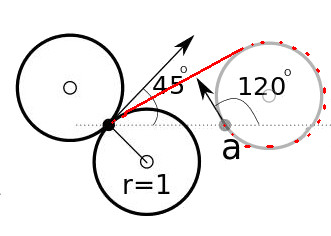
\includegraphics[width=0.5\linewidth]{img/dubinsA}
    \caption{Shortest Dubins path from $(0,0)$ to $a$}
    \label{fig_dubinsa}
\end{figure}

\subsection{}
Figure \ref{fig_dubinsb} shows the Dubins path to $b$.
\begin{figure}
    \center
    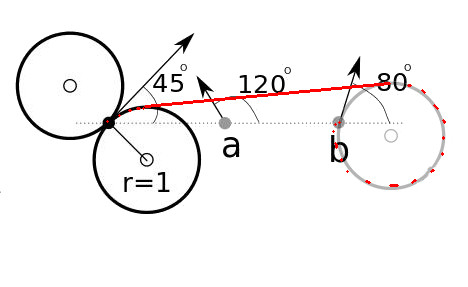
\includegraphics[width=0.5\linewidth]{img/dubinsB}
    \caption{Shortest Dubins path from $(0,0)$ to $b$}
    \label{fig_dubinsb}
\end{figure}


\section{} %4
\subsection{}

\begin{tabular}{ c }
  Front \\
  \hline
  G \\
  F \\
  D \\
  E \\
  \hline
  Back
\end{tabular}

\subsection{}

\begin{tabular}{ c }
  Front \\
  \hline
  D \\
  F \\
  B \\
  A \\
  \hline
  Back
\end{tabular}

\section{} %5
\subsection{}

Node discover order with BFS: ${F,D,G,C,E,H,A,B}$. Figure \ref{fig_bfs} shows the resulting search tree.

\subsection{}

Node discover order with DFS: ${F,D,C,A,B,E,H,G}$. Figure \ref{fig_dfs} shows the resulting search tree.

\begin{figure}
    \begin{subfigure}[t]{.49\textwidth}
        \centering
        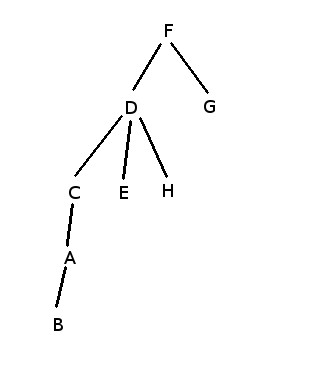
\includegraphics[width=\linewidth]{img/bfs}
        \caption{Search graph with BFS}
        \label{fig_bfs}
    \end{subfigure}\hfill
    \begin{subfigure}[t]{.49\textwidth}
        \centering
        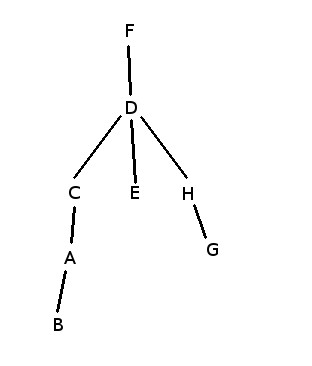
\includegraphics[width=\linewidth]{img/dfs}
        \caption{Search graph with DFS}
        \label{fig_dfs}
    \end{subfigure}
    \caption{}
\end{figure}

\end{document}